\documentclass{labreport}

\usepackage{amsmath}
\usepackage{tikz}
\usepackage{caption}
\usepackage{mathtools}
\usepackage{subcaption}
\usepackage{csquotes}
\usepackage{dirtytalk}

\usepackage{tabularx}

\title{Оценка поведения многокаскадного усилителя, охваченного обратными связями}
\subtitle{по домашней работе № 1}
\author{И.В. Бобренко}
\group{ИУ6-42Б}
\descipline{Электроника}

\begin{document}

\maketitle

\tableofcontents

\chapter{Задание}

\textbf{Вариант 35}

\begin{tabular}{|c|c|c|c|}
    \hline
    Тип диода & $Ri$, кОм & $R_\text{н}$, кОм & $C_1$, нФ \\
    \hline
    2Д231А & 4,6 & 92 & 220 \\
    \hline
\end{tabular}


\chapter{Часть 1}
\textbf{Задание}: для заданного диода найти и обосновать параметры SPICE-модели. Результат оформить в виде таблицы с объяснением соответствия найденных параметров параметрам SPICE-модели.



\begin{table}[h]
    \centering
    \begin{tabularx}{\textwidth}{|c|X|c|X|}
        Параметр & Расшифровка & Значение & Обоснование \\
        \hline
         IS &
Ток насыщения &
44,5 нА &
Из диодного уравнения \\
RS &
Паразитное сопротивление &
0.03 Ом &
Из расчётов \\
N &
Коэффициент эмиссии &
2 &
По умолчанию (для кремния) \\
TT &
Время переноса заряда &
0,05 мкс &

Исходные данные \\
CJO &
Емкость перехода при нулевом смещении &
0 Ф &
По умолчанию \\
VJ &
Контактная разность потенциалов перехода &
1 В &
По умолчанию \\
M &
Коэффициент плавности перехода &
0,5 &
По умолчанию (для лавинного перехода) \\
EG &
Ширина запрещенной зоны &
1,11 эВ &
По умолчанию (для кремния) \\
XTI &
Температурный экспоненциальный коэффициент тока насыщения &
3 &
По умолчанию (для кремния) \\
KF &
Коэффициент фликер-шума &
0 &
По умолчанию \\
AF &
Показатель степени в формуле фликер-шума &
1 &
По умолчанию \\

FC &
Коэффициент емкости обедненной области при прямом смещении &
0,5 &
По умолчанию \\

BV &
Обратное напряжение пробоя &
150 В &
Исходные данные \\
IBV & 
Обратный ток пробоя &
0,05 мА &
Исходные  данные \\



    \end{tabularx}
    \caption{Параметры модели}
    \label{tab:params}
\end{table}



\begin{gather*}
    I_S = \frac{I_D}{e^{\frac{U_D}{\varphi_T N}} - 1} = \frac{10}{e^{\frac{1}{0.052}}-1} = 4.45 \cdot 10^{-8} \\
    R_S = \frac{U_D - U_\text{откр}}{I_D} = \frac{1-0.7}{10} = 0.03
\end{gather*}

\chapter{Часть 2}

\textbf{Задание}: для заданного диода по найденным параметрам SPICE-модели построить в среде MathCAD и в среде Multisim вольтамперные характеристики для режимов прямого и обратного смещения. Сравнить полученные графики.

\begin{figure}[h]
    \centering
    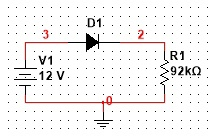
\includegraphics{ek_schema1.jpg}
    \caption{Схема электрической цепи}
\end{figure}


\begin{figure}[h]
    \centering
    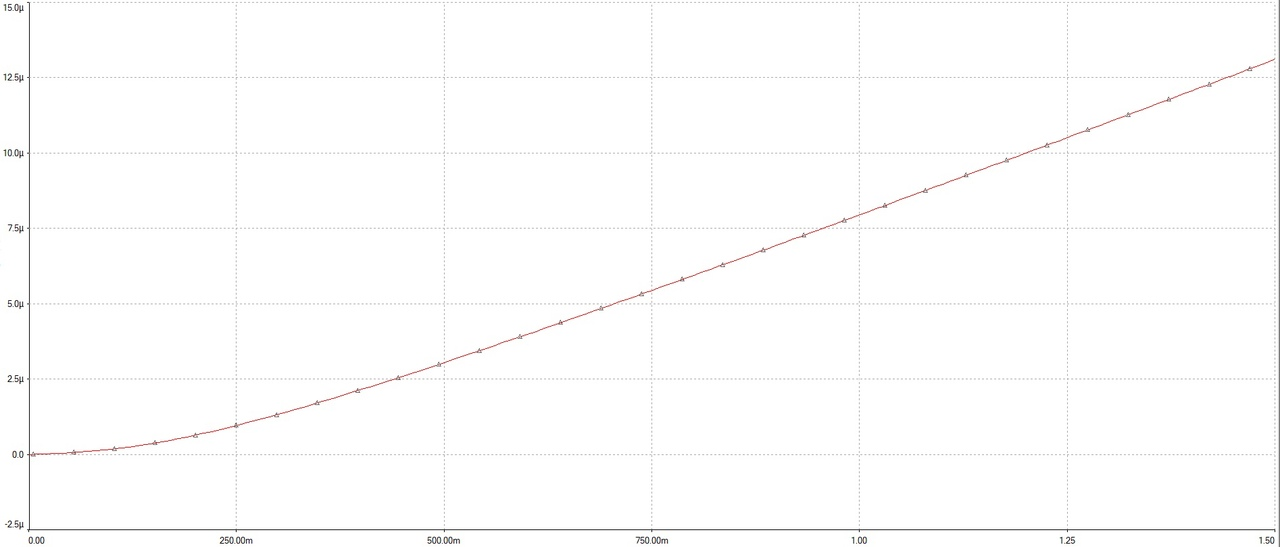
\includegraphics[width=\linewidth]{ek_graph_pos_m.jpg}
    \caption{Положительная ВАХ в Multisim}
\end{figure}


\begin{gather}
    I_D=I_S\cdot\left(e^{\frac{U_D}{\varphi_TN}}-1\right)
    \label{for:1}
\end{gather}

\begin{gather}
    I_D \approx \frac{I_S}{1-\left( \frac{U_D}{U_{BV}} \right)^K}
    \label{for:2}
\end{gather}
\begin{figure}[h]
    \centering
    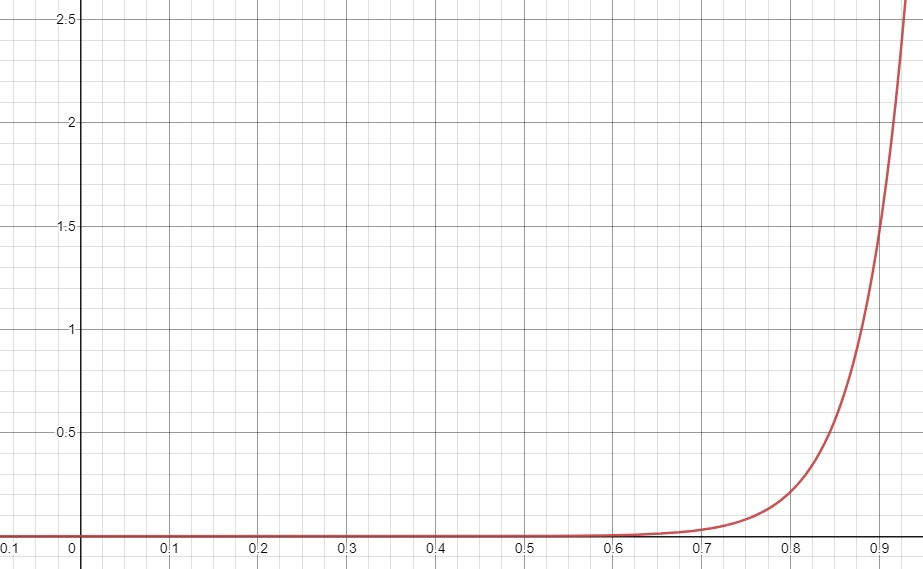
\includegraphics[width=\linewidth]{ek_graph_pos_a.jpg}
    \caption{Положительная ВАХ аналитическая по формуле \ref{for:1}}
\end{figure}




\begin{figure}[h]
    \centering
    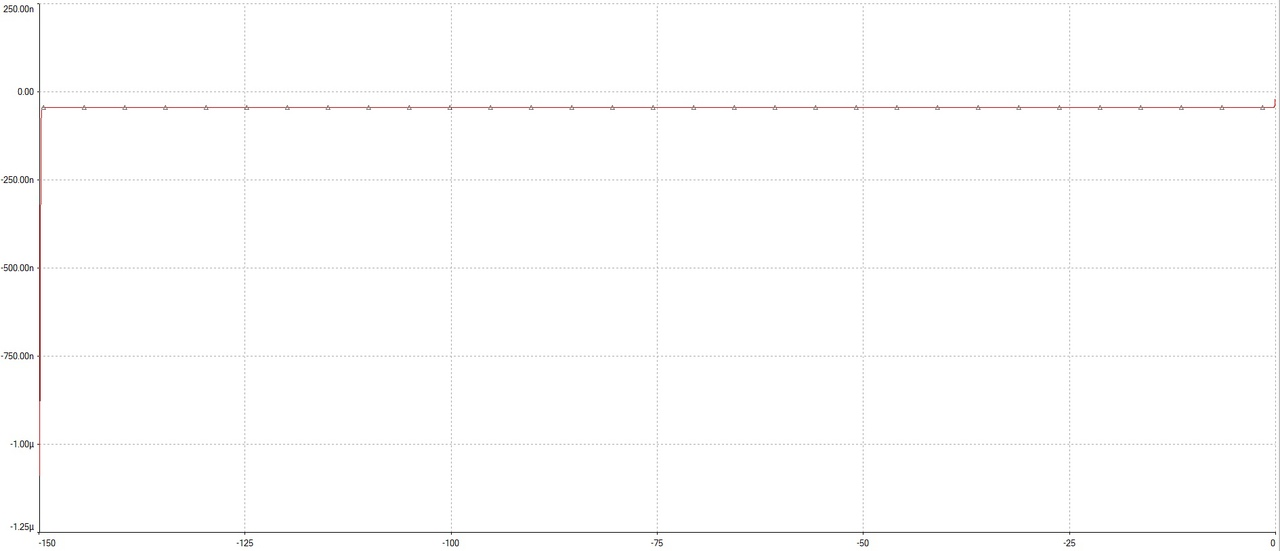
\includegraphics[width=\linewidth]{ek_graph_neg_m.jpg}
    \caption{Отрицательная ВАХ в Multisim}
\end{figure}

\begin{figure}[h]
    \centering
    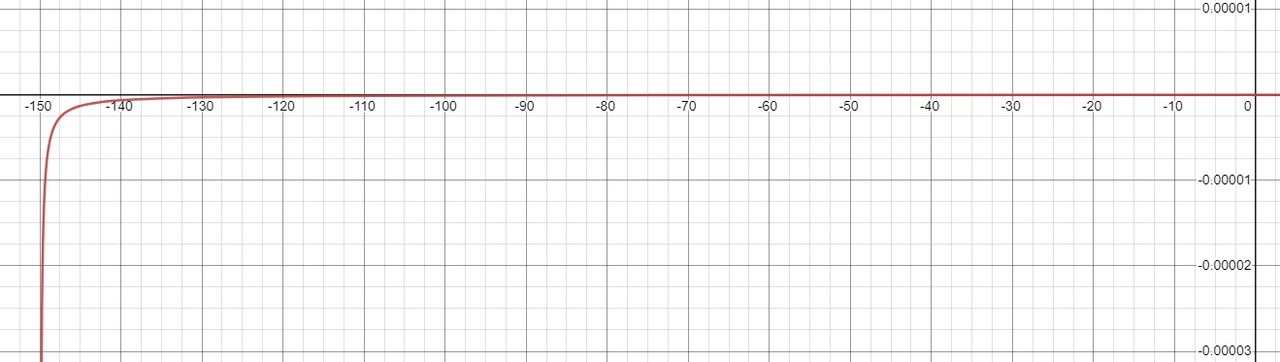
\includegraphics[width=\linewidth]{ek_graph_neg_a.jpg}
    \caption{Отрицательная ВАХ аналитическая по формуле \ref{for:2}}
\end{figure}


В среде Multisim учитывается сопротивление диода, из-за чего график стремится к прямой, в отличие от графика, полученного аналитически, который представляет собой экспоненту.

\chapter{Часть 3}
\textbf{Задание:} для схемы из пункта 2 найти и построить зависимости тока, напряжения на диоде и выходного напряжения от входного напряжения в диапазоне от 0 до 10В: 
\begin{enumerate}
    \item  графическим методом наложения характеристик. Использовать лист миллиметровой бумаги размером А4. Шаг по напряжению 1. 
    \item  в среде Multisim. 
\end{enumerate}
    
Заданы: напряжение $E$ и сопротивление $R$ эквивалентного источника $U_\text{вх}$, сопротивление $R_\text{н}$ нагрузки. Использовать нелинейную модель диода. Сравнить полученные результаты.


\begin{figure}[h]
    \centering
    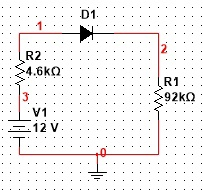
\includegraphics{ek_schema2.jpg}
    \caption{Схема электрической цепи}
\end{figure}

\begin{figure}[h]
    \centering
    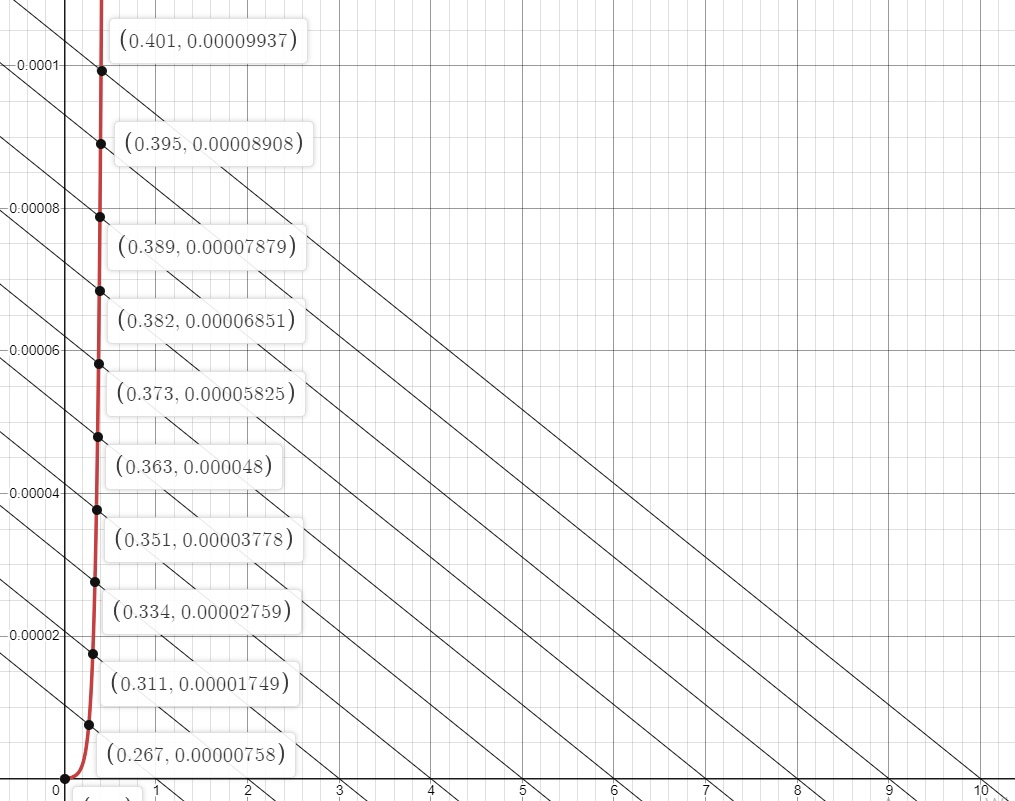
\includegraphics[width=\linewidth]{ek_lay_graph.jpg}
    \caption{Метод наложения}
\end{figure}




\begin{figure}[h]
    \centering
    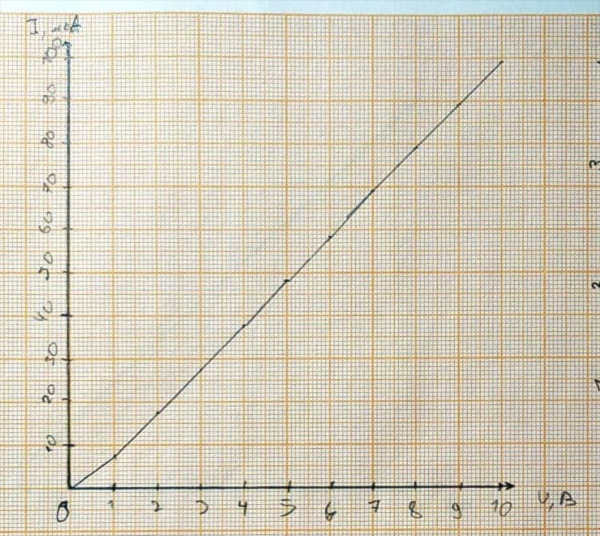
\includegraphics[width=\linewidth]{graph_h_i.png}
    \caption{Зависимость тока на диоде от напряжения}
\end{figure}

\begin{figure}[h]
    \centering
    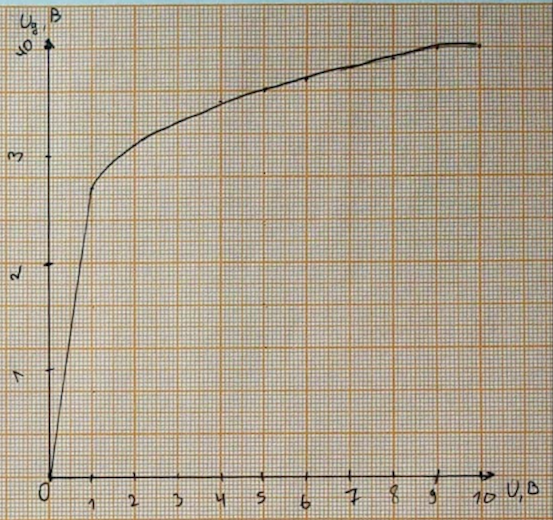
\includegraphics[width=\linewidth]{graph_h_u_d.png}
    \caption{Зависимость напряжения на диоде от напряжения}
\end{figure}

\begin{figure}[h]
    \centering
    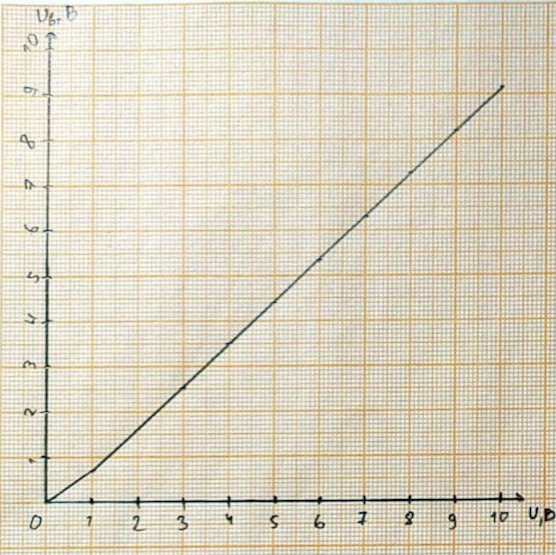
\includegraphics[width=\linewidth]{graph_h_u_o.png}
    \caption{Зависимость напряжения на выходе от напряжения}
\end{figure}


\begin{figure}[h]
    \centering
    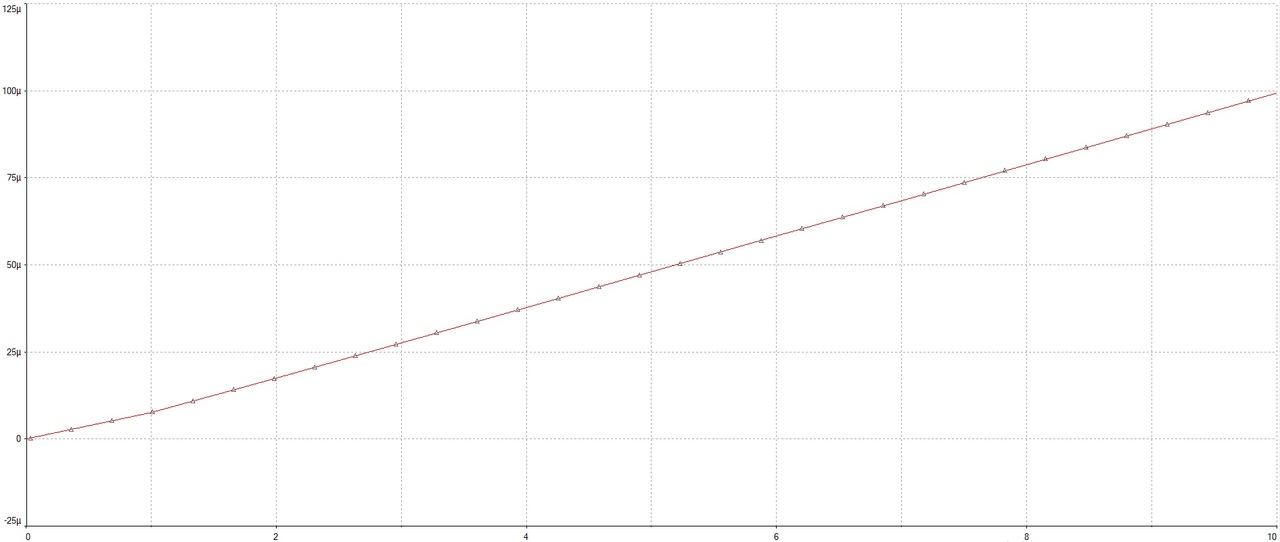
\includegraphics[width=\linewidth]{graph_m_i_d.jpg}
    \caption{Ток на диоде}
\end{figure}

\begin{figure}[h]
    \centering
    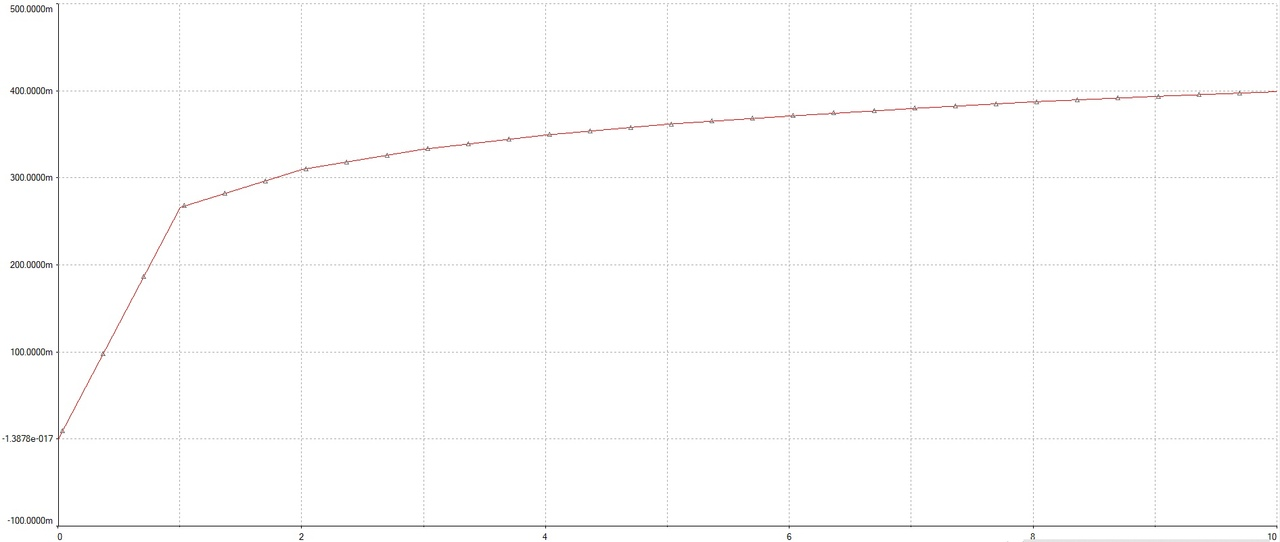
\includegraphics[width=\linewidth]{graph_m_u_d.jpg}
    \caption{Напряжение на диоде}
\end{figure}

\begin{figure}[h]
    \centering
    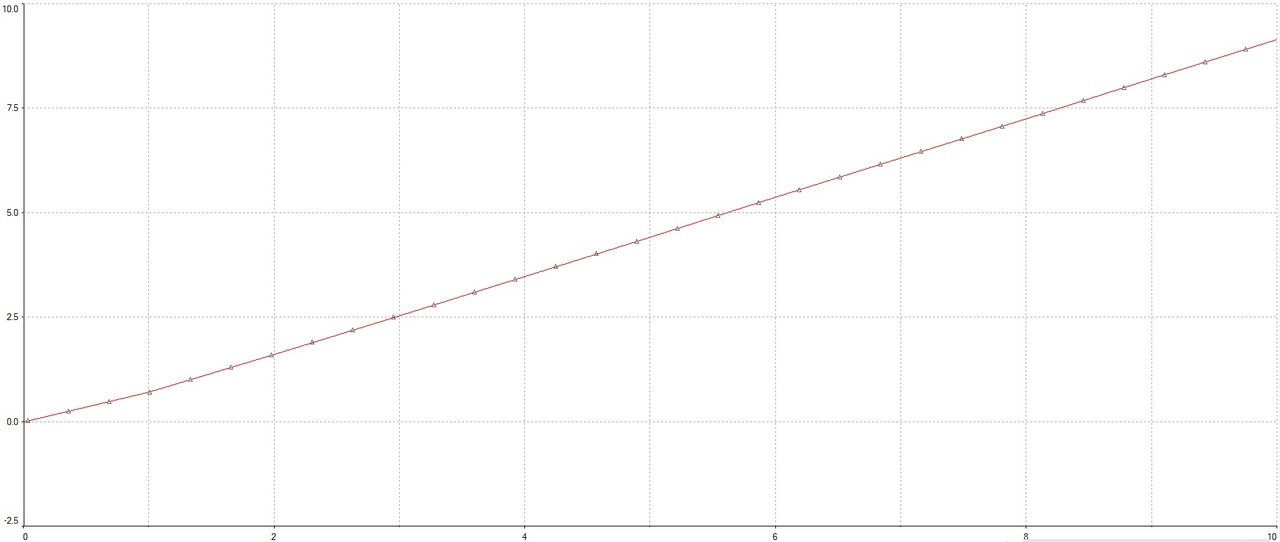
\includegraphics[width=\linewidth]{graph_m_u_o.jpg}
    \caption{Напряжение на выходе}
\end{figure}



Графики, полученные с использованием Multisim, представляют собой идеальные линии, в отличие от графиков, построенных по точкам, в связи с наличием погрешности от построений от руки.


\chapter{Часть 4}
Задание: для заданной схемы найти и построить зависимость выходного напряжения от времени при подаче на вход знакопеременного симметричного меандра с амплитудой 10В и частотой 1 кГц на протяжении двух периодов меандра: 
\begin{enumerate}
    
    \item Аналитически любым методом в среде MathCAD.
    \item В среде Multisim. Использовать кусочно-линейную модель ВАХ диода.
\end{enumerate}

Сопротивлением открытого p-n перехода пренебречь. Сравнить полученные результаты. Найти и сравнить полученные средние значения выходного напряжения и размах пульсаций p-p.

\begin{figure}[h]
    \centering
    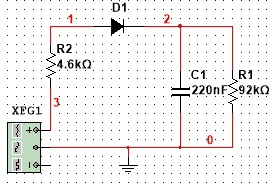
\includegraphics{ek_schema3.jpg}
    \caption{Схема электрической цепи}
\end{figure}

\section{Операторный метод}
Характеристическое уравнение для первого полупериода:
\begin{gather}
    Z_\text{вх} = R_2 + \frac{R_1}{p_1C\left( R_1 + \frac{1}{p_1C} \right)} = 0 \\
    \frac{R_1}{p_1C\left( R_1 + \frac{1}{p_1C} \right)} = -R_2 \\
    \frac{R_1}{p_1C} = -R_2\left( R_1 + \frac{1}{p_1C} \right) \\
    \frac{R_1}{p_1C} + \frac{R_2}{p_1C} = -R_2R_1 \\
    \frac{1}{p_1C} = \frac{-R_2R_1}{R_1+R_2} \\ 
    p_1 = \frac{-R_1+R_2}{R_1R_2C} \\
    U_\textit{вых св} = A_1e^{p_1t} \\ 
    U_\textit{вых пр} = \frac{R_1}{R_2+R_1}E \\ 
    U_\textit{вых полн} =  U_\textit{вых пр}(0)+ U_\textit{вых св}(0) \\ 
    0 = \frac{R_1}{R_2+R_1}E+A_1e^{p_1\cdot 0} \\ 
    A_1 = \frac{-R_1}{R_2+R_1}E \\
    U_{\text{вых}_1}(t) = \frac{R_1}{R_2+R_1}E - \frac{R_1}{R_2+R_1}Ee^{\frac{-R_1+R_2}{R_2R_1C}t}
\end{gather}

Для второго полупериода:
\begin{gather}
    Z_\text{вх} = R_1 + \frac{1}{p_2C} = 0 \\
    p_2 = - \frac{1}{R_1C} \\
    U_\textit{вых св} = A_2e^{p_2t} \\ 
    U_\textit{вых пр} = 0 \\ 
    U_\textit{вых полн} =  U_{\textit{вых}_1}(t_1)+ U_\textit{вых св}(0) \\ 
    A_2 = U_{\textit{вых}_1} (t_1)\\
    U_{\textit{вых}_2}(t) = U_{\textit{вых}_1}(t_1)e^{\frac{-1}{R_1C}(t-t_1)}
\end{gather}

Для третьего:
\begin{gather}
    Z_\text{вх} = R_2 + \frac{R_1}{p_3C\left(R_1+\frac{1}{p_3C}\right)} = 0 \\
    p_3 = p_1 = \frac{R_2-R_1}{R_1R_2C} \\
    U_\textit{вых св} = A_3e^{p_3t} \\ 
    U_\textit{вых пр} = \frac{R_1}{R_2+R_1}E \\ 
    U_\textit{вых полн} =  U_{\textit{вых}_2}(t_2) =U_\textit{вых пр}(0) + U_\textit{вых св}(0) \\ 
    A_3 = U_{\textit{вых}_2} (t_2) - \frac{R_1}{R_2+R_1}E\\
    U_{\textit{вых}_3}(t) = \frac{R_1}{R_2+R_1}E + \left(U_{\textit{вых}_2}(t_2)-\frac{R_1}{R_2+R_1}E\right)e^{\frac{R_2-R_1}{R_1R_2C}(t-t_2)}
\end{gather}

Для четвёртого:
\begin{gather}
    Z_\text{вх} = R_1 + \frac{1}{p_4C} = 0 \\
    p_4 = p_2 = - \frac{1}{R_1C} \\
    U_\textit{вых св} = A_4e^{p_4t} \\ 
    U_\textit{вых пр} = 0 \\ 
    U_\textit{вых полн} =  U_{\textit{вых}_3}(t_3)+ U_\textit{вых св}(0) \\ 
    A_4 = U_{\textit{вых}_3} (t_3) \\
    U_{\textit{вых}_4}(t) = U_{\textit{вых}_3}(t_3)e^{\frac{-1}{R_1C}(t-t_3)}
\end{gather}

\section{Графики}

\begin{samepage}
\begin{figure}[h]
    \centering
    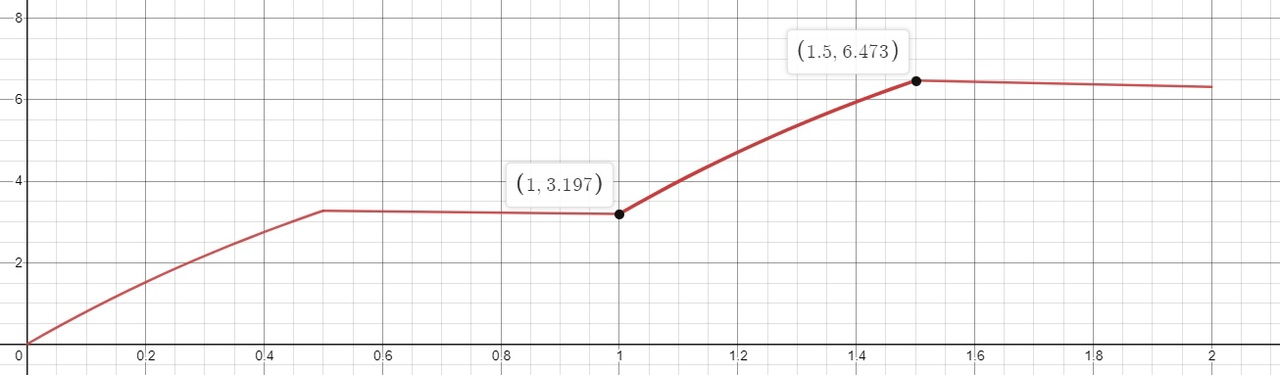
\includegraphics[width=\linewidth]{graph_x_a.jpg}
    \caption{График переходного процесса аналитический}
\end{figure}

Минимальное значение $= 0$ В

Максимальное значение $= 6,473$ В

Среднее значение $= 3,237$ В

Размах пульсаций $= 6,473 - 3,197 = 3,276$ В

\end{samepage}


\begin{samepage}
\begin{figure}[h]
    \centering
    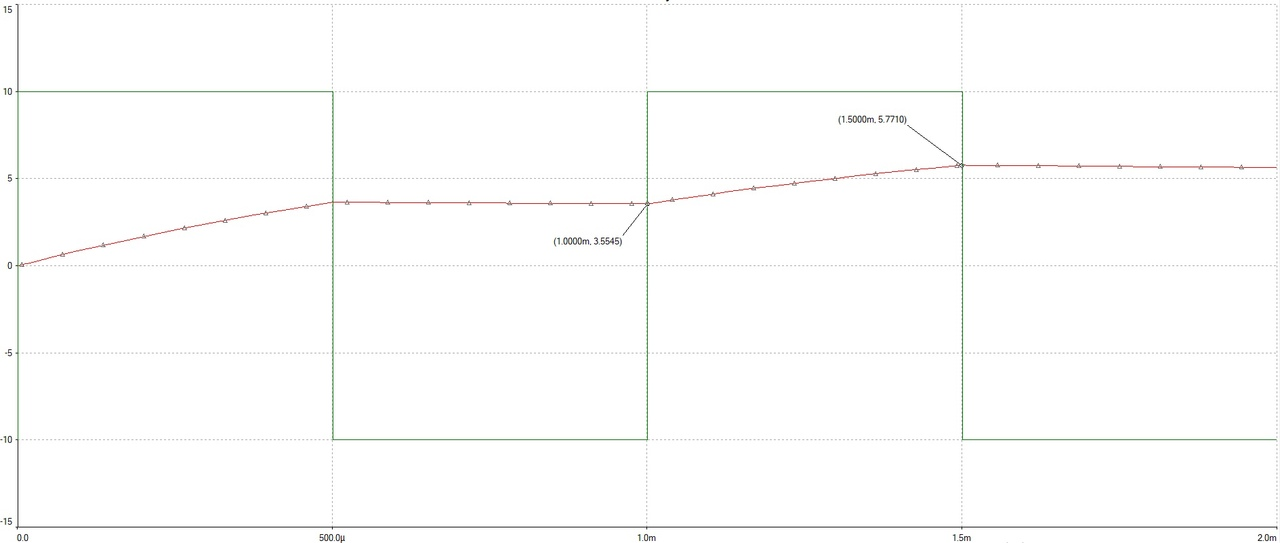
\includegraphics[width=\linewidth]{graph_x_m.jpg}
    \caption{График переходного процесса в Multisim}
\end{figure}

Минимальное значение $= 0$ В

Максимальное значение $= 5,7710$ В

Среднее значение $= 2,8855$ В

Размах пульсаций $= 5,7710 - 3,5545 = 2,2165$ В

\end{samepage}







\chapter{Выводы}
Модель диода с большой точностью описывает реальный образец, однако не учитывает некоторые физические параметры (как, например, паразитное сопротивление), из-за чего теоретическая и реальная ВАХ отличаются.

Зависимости тока на диоде, напряжения на диоде и напряжения на выходе с большой точностью совпадают с полученными программным путём. Следовательно, расчёты выполнены преимущественно верно.

Зависимости напряжения на выходе от времени при подаче на вход симметричного знакопеременного меандра, полученные операторным методом и программным способом, похожи с большой долей точности. Расхождения в конкретных значениях обусловлены тем фактом, что в программе Multisim используется линейная модель диода, в то время как в расчётах была использована нелинейная.
\section{Сипсок использованных источников:}

\begin{itemize}
    \item Электронная техника, 2004 -- Москатов Е.А. 
    \item Справочник по полупроводниковым приборам, 2011 -- Москатов Е.А. 
    \item Электроника и микропроцессорная техника: учебник для вузов, 2013. -- Гусев В.Г., Гусев Ю.М. 
\end{itemize}
    
\end{document}
